\documentclass[10pt,a4paper]{article}
\usepackage[T1]{fontenc}
\usepackage{lmodern,microtype}
\usepackage[margin=23mm]{geometry}
\usepackage{amsmath,amssymb,graphicx,booktabs,tabularx,longtable,array}
\usepackage[table]{xcolor}
\usepackage{enumitem,float,caption,xurl,listings,circuitikz}
\usepackage[numbers,sort&compress]{natbib}
\usepackage[colorlinks=true,allcolors=blue!50!black]{hyperref}
\usetikzlibrary{positioning,arrows.meta,shapes.geometric}
\setlist{nosep,leftmargin=*}
\setlength{\parskip}{4pt}
\setlength{\parindent}{1em}
\widowpenalty=10000\clubpenalty=10000
\renewcommand{\tabularxcolumn}[1]{>{\raggedright\arraybackslash}p{#1}}
\renewcommand{\arraystretch}{1.15}
\captionsetup{font=small,labelfont=bf}
\hypersetup{pdftitle={CrashGuard: Crash Detection and Emergency Alerts},pdfauthor={Adheesh Garg, Ayan Gatani, Aastha Gupta, Syamasudha Veeragandham}}
\bibliographystyle{IEEEtran}
\lstset{basicstyle=\ttfamily\small,breaklines=true,columns=fullflexible,frame=single}
\newcommand{\degree}{\ensuremath{^{\circ}}}
\newcommand{\fig}[3]{\begin{figure}[H]\centering\includegraphics[width=#2\linewidth]{#1}\caption{#3}\end{figure}}
\begin{document}
\begin{center}
{\LARGE\bfseries CrashGuard: Simulation-Based Evaluation of an IoT Crash Detection and Emergency Alert System for Two-Wheeler Riders\par}
\vspace{6mm}
Adheesh Garg\textsuperscript{1}, Ayan Gatani\textsuperscript{1}, Aastha Gupta\textsuperscript{1},\\
Syamasudha Veeragandham\textsuperscript{2,*}\\[3mm]
\textsuperscript{1,2}School of Computer Science and Engineering,\\
Vellore Institute of Technology, Vellore, Tamil Nadu, India -- 632014\\[3mm]
{\small\href{mailto:adheesh.garg2023@vitstudent.ac.in}{adheesh.garg2023@vitstudent.ac.in}\\
\href{mailto:ayan.gatani2023@vitstudent.ac.in}{ayan.gatani2023@vitstudent.ac.in}\\
\href{mailto:aastha.gupta2023@vitstudent.ac.in}{aastha.gupta2023@vitstudent.ac.in}\\
\textsuperscript{*}Corresponding author: \href{mailto:syamasudha.v@vit.ac.in}{syamasudha.v@vit.ac.in}}\\[3mm]
{\small Programming for IoT Boards}
\end{center}
\begin{abstract}
CrashGuard detects motorcycle crash-like motion using a handlebar-mounted ESP32 and MPU-6050, activates a local alarm, and provides a 15-second rider cancellation interval before an IoT event. This study evaluates the implemented state machine through reproducible six-axis simulation, public motorcycle signal analysis, and execution of the firmware with virtual peripherals. The detector combines ride qualification, impact or unloading, correlated angular motion, and sustained tilted rest. A deterministic 675-event replay produced 94.7\% accuracy, 76.0\% sensitivity, 100.0\% observed specificity, and an F1-score of 0.864. A fresh 270-event simulation with unchanged thresholds produced 93.7\% accuracy, 71.7\% sensitivity, 100.0\% observed specificity, and an F1-score of 0.835. On the fresh set, acceleration-only detection generated 108 false positives, while CrashGuard generated none and missed 17 low-side events. The median candidate-to-confirmation delay was 2.33 seconds. Fourteen executable firmware scenarios exercised calibration, sensor failures, alarm timing, cancellation, cloud submission, and communication outages. Fault injection exposed rest-timer continuity across missing samples, a five-second cloud timeout, and one-shot delivery without recovery retry. A time-stepped battery simulation yielded 12.64 hours at a 120 mA, 5 V load and 90\% conversion efficiency. Circuit, architecture, flowchart, virtual-hardware visualization, data partitions, algorithms, metrics, and logs accompany the results. The findings establish reproducible simulation performance and identify specific changes needed to improve low-energy detection and fault recovery.
\end{abstract}
\noindent\textbf{Keywords:} IoT; ESP32; MPU6050; Motorcycles; Detection; Simulation; Alerts; Safety.
\clearpage

\section{Introduction}
Boubezoul et al. (2013) established a motorcycle-specific fall-detection reference~\cite{boubezoul2013algorithm}. Their work places the detection problem within powered-two-wheeler dynamics. This domain includes large lean angles and disturbances during ordinary riding. Consequently, a brief acceleration peak cannot fully characterize an accident. The paper motivates examining the sequence surrounding a suspected fall. For CrashGuard, the relevant gap is translating this need into inspectable firmware. We combine riding context, inertial corroboration, and sustained final posture. Each intermediate decision is represented by an explicit state transition. Our evaluation compares this sequence with two simpler executable rules. The measured improvement concerns false-alarm rejection on the same simulation data.


Boubezoul et al. (2019) released public motorcycle fall and critical-event recordings~\cite{boubezoul2019dataset}. This contribution makes independent inspection of representative signals possible. Positive events describe falls, while critical manoeuvres challenge specificity. The recordings provide an external reference for acceleration and rotation scale. A remaining evaluation need is to distinguish gate crossings from a full decision. CrashGuard processes four fall recordings and seven critical manoeuvres. We publish the conversion, filtering, resampling, and selected time windows. Individual gates are evaluated separately from ride qualification and final rest. All four fall windows cross the unloading and rotation gates used by our detector. This analysis improves threshold traceability without treating crossings as accuracy.


Gelmini et al. (2021) investigated crash detection for two-wheeled vehicles~\cite{gelmini2021novel}. Their study reinforces the importance of evaluating diverse vehicle behaviour. A detector must accommodate substantial differences between accidents and riding. The vehicle domain therefore demands more than one convenient positive example. For our prototype, a key gap is scenario coverage in a reproducible small platform. CrashGuard evaluates braking, turning, road shocks, recovery, and parked tip-over. Low-side and high-side events are retained as separate positive categories. This separation reveals which motion family accounts for missed detections. Every fresh high-side event is detected, whereas seventeen low-side events are missed. Our contribution is a transparent error breakdown rather than cross-study superiority.


Sucerquia et al. (2017) introduced SisFall for human falls and everyday activities~\cite{sisfall}. The dataset uses a waist-mounted device and includes a broad activity collection. Its methodological value is the deliberate inclusion of non-fall motion. Testing only positive events would conceal nuisance alarms during ordinary use. The transfer gap is that human-body recordings differ from handlebar measurements. CrashGuard therefore constructs negative scenarios that describe motorcycle motion. Seven negative classes are evaluated alongside two positive fall-like classes. Event labels and class counts remain visible in the published result tables. On the fresh simulation, the detector rejects all 210 negative events. The improvement is explicit negative-event coverage within the intended signal model.


Casilari et al. (2017) analyzed public datasets for wearable fall detection~\cite{survey}. Their comparison highlights variation in sensors, activities, and collection protocols. Such differences affect what a reported accuracy or sensitivity can establish. A detector evaluated on one recording setup may face a different signal distribution. The methodological gap is incomplete reporting of how evaluation data are constructed. CrashGuard publishes channel units, sampling rates, seeds, labels, and scenario counts. The generator also specifies bias, noise, clipping, and the motion trajectories. Whole events remain together when assigning development, validation, and test subsets. A separate random stream adds a repeatability check with unchanged detector settings. This improves experimental transparency while retaining the limits of the signal model.


Casilari et al. (2020) evaluated convolutional models across public fall datasets~\cite{cnn}. Their study emphasizes the influence of the selected repository on classifier results. This motivates distinguishing repeatability within a domain from transfer across domains. A new random seed alone does not create a different vehicle or mounting distribution. CrashGuard therefore describes the fresh dataset as a same-generator evaluation. The public motorcycle recordings supply a separate analysis of physical signal scale. We report these two forms of evidence in distinct tables with distinct endpoints. This avoids combining gate crossings with complete event-classification outcomes. Future evaluation should hold out whole vehicle sessions and mounting configurations. The present contribution is a clear separation of evidence and a reproducible comparison.


Musci et al. (2018) studied online fall detection using recurrent neural networks~\cite{musci}. Their LSTM classifier uses temporal information from annotated SisFall sequences. This supports examining motion over time instead of treating samples independently. A learned sequence model and an explicit state machine encode timing differently. Our engineering need is a compact decision path that can be inspected during faults. CrashGuard uses correlation windows, verification timeouts, and a rest-hold timer. The same detector implementation serves both native replay and the firmware. This removes a separate reimplementation as a source of evaluation disagreement. Fault injection can then connect an observed outcome to a particular transition. The resulting contribution is reproducible temporal logic with identifiable failures.


Yu et al. (2021) introduced KFall with temporal labels for pre-impact detection~\cite{kfall}. Their work makes the timing objective an explicit part of algorithm evaluation. Pre-impact protection and post-event notification require different response times. The timestamp used as the start of a delay measurement therefore matters. For CrashGuard, the reporting gap is distinguishing confirmation from notification. We report candidate-to-confirmation time independently of the cancellation interval. The fresh-event median confirmation delay is 2.33 seconds among detected positives. A further fifteen seconds gives the rider an opportunity to cancel the warning. The firmware harness checks the exact deadline and the cancellation response. This provides a traceable timing contract for the post-event alert application.


Rodegast et al. (2024) investigated machine learning for motorcycle collision detection~\cite{rodegast2024}. Their study uses simulated accidents and riding operation to develop classifiers. Its application requires rapid collision recognition for passive safety activation. The authors emphasize avoiding false activation across impact configurations. That objective differs from a cancellable warning after a fall-like event. CrashGuard uses simulation to evaluate a slower post-event notification sequence. The fresh dataset is generated after freezing the rules for the current study. Both comparison rules receive exactly the same input events as our detector. This exposes the measured balance between missed events and nuisance warnings. Our additional focus is the executable alarm and fault path surrounding classification.


Leoni et al. (2025) proposed a dynamics-based automatic eCall method for motorcycles~\cite{ecall2025}. Their study considers both rapid high-side motion and slower side-slip behaviour. This distinction directly motivates separate analysis of high- and low-energy falls. A single response scale can favour one accident family while missing another. CrashGuard addresses the reporting gap by retaining both families in every split. Its threshold sequence produces strong rejection of the generated non-crash events. The fresh low-side recall remains weaker and is reported as the main detector gap. We therefore avoid presenting high overall accuracy as evidence of uniform protection. The observed class-specific misses identify where adaptive dynamics could help. Our practical contribution is an auditable implementation and targeted improvement plan.


Tian et al. (2026) proposed multi-head attention for shinbone-mounted fall detection~\cite{tian2026transformer}. The paper combines temporal representation learning with a wearable implementation. Its reported test sensitivity is 90.5 percent, with 93.1 percent overall accuracy. The study also highlights the influence of class imbalance on fall recognition. The transfer gap is the difference between human-leg and motorcycle-handlebar motion. CrashGuard retains this study as recent sequence-learning context for its design. We report positive and negative counts, F1, and sensitivity alongside accuracy. Our classifier adds a rider cancellation interval and an instrumented IoT event path. Firmware simulations connect the inertial decision to local outputs and service calls. These are integration contributions, not a claim to outperform the human-fall model.


Pradhan et al. (2026) introduced a dual-stream transformer with Kalman sensor fusion~\cite{dual2026}. The model uses complementary inertial information for wearable fall recognition. Its SmartFallMM evaluation reports an F1-score of 91.10 percent. The subject-wise evaluation also addresses variation between individual participants. This recent work motivates richer fusion and stronger separation of evaluation groups. CrashGuard currently combines three interpretable inertial features through fixed rules. Its contribution is a lightweight sequence linked to directly observable alert states. We preserve whole events within partitions and evaluate an additional random stream. Future vehicle- and session-wise splits would test a stronger form of generalization. The comparison identifies a next step without equating different datasets or devices.


\subsection{Research gaps and demonstrated improvements}
The literature motivates three specific engineering gaps for this implementation: amplitude-only decisions admit road disturbances, event accuracy alone omits alert-chain failures, and a single aggregate score can conceal weaker low-side detection. CrashGuard addresses the first with ride qualification and temporal corroboration, the second with an executed sensor-to-alarm-to-service harness, and the third with class-specific reporting on a separate random stream. These contributions concern the evaluated prototype and do not imply that every cited system omits the same functions.

The direct improvement is established against the two rules evaluated on identical data. On the fresh set, CrashGuard eliminates 108 acceleration-only false positives and detects 30 more positives than the strict ordered rule. Its local warning, fifteen-second cancellation contract, published replay data, and fourteen fault-oriented firmware cases add implementation evidence beyond those baseline decision rules. The cost is nine additional misses relative to acceleration-only detection; low-side recall, sample freshness, and eventual delivery remain explicit improvement targets.

\subsection{Research Objectives}
\begin{enumerate}
\item Implement and evaluate a 100 Hz, six-axis state machine for handlebar-mounted crash-like event detection, with local warning and rider cancellation.
\item Compare the frozen detector with acceleration-only and strict ordered rules using deterministic and fresh-seed event sets, reporting confusion counts, sensitivity, specificity, F1, and delay.
\item Exercise sensor, calibration, timing, and communication failures by running the firmware with controlled virtual peripherals and recording expected versus actual behavior.
\item Provide reproducible datasets, plots, circuit and architecture diagrams, power simulation, and a traceable account of limitations and future improvements.
\end{enumerate}

\section{Related Work}
Boubezoul et al. studied a simple fall detection algorithm for powered two-wheelers~\cite{boubezoul2013algorithm}. Its importance here is the direct vehicle domain: a detector must respond to the motion of the motorcycle, including conditions that resemble a fall. CrashGuard follows this domain focus while evaluating a different explicit sequence of acceleration, rotation, and final rest.

Boubezoul et al. subsequently published a dataset of powered-two-wheeler falls and critical events~\cite{boubezoul2019dataset}. Its open recordings support reproducible signal inspection. The present work processes four falls and seven critical manoeuvres, compares threshold crossings, and keeps those measurements separate from the generated event-classification dataset.

Gelmini et al. investigated crash detection for two-wheeled vehicles using experimental riding data~\cite{gelmini2021novel}. This work emphasizes the breadth of vehicle behavior that a practical detector must accommodate. It motivates inclusion of braking, cornering, road disturbances, recovery, and different fall profiles in CrashGuard's scenario design.

Sucerquia et al. introduced SisFall, a waist-mounted dataset containing falls and activities of daily living~\cite{sisfall}. Its structured non-fall activities illustrate why a positive-only evaluation is insufficient. CrashGuard applies that evaluation principle to a different domain by including seven negative motorcycle scenarios alongside two positive scenarios.

Casilari et al. analyzed public datasets for wearable fall detection~\cite{survey}. Differences in sensor location, sampling, activity composition, and protocol affect the interpretation of results. This motivates publishing the complete sampling rate, channel units, scenario distributions, random seeds, and event-level partitions in the present study.

Musci et al. developed online fall detection using recurrent neural networks and evaluated an LSTM-based classifier on SisFall with extended annotation~\cite{musci}. Their use of temporal structure provides a useful methodological comparison. CrashGuard encodes temporal structure with a finite-state detector whose intermediate decisions can be checked without neural training.

Tian et al. proposed a multi-head attention transformer for a shinbone-mounted human-fall device~\cite{tian2026transformer}. The paper reports 90.5\% test sensitivity and 93.1\% overall accuracy after balancing and focal-loss training. Those values contextualize sequence learning; the different mounting, labels, population, and protocol preclude treating them as a common-dataset ranking against CrashGuard.

Yu et al. introduced KFall with synchronized temporal labels and benchmark algorithms for pre-impact fall detection~\cite{kfall}. Their work highlights the importance of stating where timing begins and ends. CrashGuard reports candidate-to-confirmation delay and the subsequent cancellation interval explicitly, since its intended behavior is post-event notification.

Casilari et al. evaluated convolutional neural networks across multiple public fall datasets~\cite{cnn}. Their findings show why a classifier's score should be interpreted with its data source. CrashGuard's fresh-seed experiment checks repeatability within the same generator family, while the public motorcycle analysis checks signal scale in a separate source domain.

Blynk's device-template and event documentation describes the device identity, event code, and firmware submission operation used for an IoT event~\cite{blynktemplate,blynkevents}. This platform work complements detection research by defining the controller-to-cloud interface. CrashGuard exercises that interface with a deterministic local event sink and records submission, disconnection, and timeout outcomes separately.

Rodegast et al. (2024) evaluate learned motorcycle collision detection using accident and riding simulations~\cite{rodegast2024}. Their passive-safety objective prioritizes rapid detection without false activation. CrashGuard instead evaluates a post-event warning with rider cancellation. The shared lesson is to match evaluation metrics and timing endpoints to the intended intervention.

Leoni et al. (2025) address motorcycle eCall using a dynamics-based method~\cite{ecall2025}. Their distinction between high-frequency high-side motion and slower side slips is particularly relevant to CrashGuard's low-side misses. It motivates adding richer dynamics while preserving a fixed, reproducible negative-event benchmark.

Pradhan et al. (2026) combine dual-stream transformer processing with Kalman-based inertial fusion~\cite{dual2026}. Their 21-fold leave-one-subject-out SmartFallMM evaluation reports 91.10\% F1. This recent approach motivates future fusion and group-wise evaluation, while CrashGuard contributes directly inspectable state transitions and alert-path fault characterization in the motorcycle simulation domain.

The following comparison organizes prior work by sensing domain, inference method, and its specific relationship to CrashGuard. It separates direct motorcycle references from human-fall methodology and the cloud interface, so that the reader can identify which design choice each source informs.

\small
\begin{longtable}{@{}>{\raggedright\arraybackslash}p{.21\linewidth}>{\raggedright\arraybackslash}p{.25\linewidth}>{\raggedright\arraybackslash}p{.46\linewidth}@{}}
\caption{Comparison of prior motorcycle-crash, human-fall, dataset, and IoT-interface research and its specific role in CrashGuard. The first column identifies the source, the second states its sensing domain or analytical method, and the third explains the design or evaluation decision informed by that source. Public motorcycle data provide an external signal reference; human-fall studies inform methodology but use different mounting positions and labels. The rows describe methodological relationships, not a common-dataset performance ranking.}\label{tab:prior}\\
\toprule
Source & Sensing domain / method & Specific relevance and evaluation boundary\\\midrule\endfirsthead
\toprule Source & Sensing domain / method & Specific relevance and evaluation boundary\\\midrule\endhead
Boubezoul et al. (2013)~\cite{boubezoul2013algorithm} & Motorcycle fall algorithm & Motivates motorcycle-specific temporal decisions; our implementation exposes the candidate, rotation, and rest states for direct replay.\\
Boubezoul et al. (2019)~\cite{boubezoul2019dataset} & Public PTW recordings & Supplies four controlled falls and seven critical manoeuvres. We retain their original labels and evaluate filtered acceleration and rotation gates separately.\\
Gelmini et al. (2021)~\cite{gelmini2021novel} & Motorcycle crash detection & Motivates evaluation across different vehicle behaviours. Our scenarios retain braking, turning, road shocks, and recovery as explicit negative classes.\\
SisFall (2017)~\cite{sisfall} & Waist inertial dataset & Demonstrates the importance of everyday non-fall examples. We transfer this evaluation principle to motorcycle scenarios, not the human-body labels.\\
Casilari et al. (2017)~\cite{survey} & Dataset analysis & Motivates disclosure of sensor location, sampling rate, units, event composition, and split procedure to make performance claims interpretable.\\
Musci et al. (2018)~\cite{musci} & Online LSTM detection & Provides a learned temporal-recognition reference. CrashGuard instead makes its correlation and rest timing explicit in a fixed-rule state machine.\\
Tian et al. (2026)~\cite{tian2026transformer} & Shinbone transformer & Provides recent attention-based human-fall context and illustrates sensitivity to class balance. The shinbone mounting differs from our handlebar location.\\
KFall (2021)~\cite{kfall} & Pre-impact timing dataset & Separates pre-impact timing from post-event detection. We report candidate-to-confirmation delay independently of the later cancellation interval.\\
Casilari et al. (2020)~\cite{cnn} & Multi-dataset CNN study & Motivates separating a fresh random stream from a different acquisition domain. Our public PTW analysis and synthetic classification results remain distinct.\\
Rodegast et al. (2024)~\cite{rodegast2024} & Simulated motorcycle collision learning & Investigates simulated motorcycle collisions for rapid protective-system activation. Our application instead evaluates a cancellable post-event warning.\\
Leoni et al. (2025)~\cite{ecall2025} & Dynamics-based motorcycle eCall & Distinguishes rapid high-side motion from slower side-slip dynamics, directly motivating the separate reporting of CrashGuard low-side misses.\\
Pradhan et al. (2026)~\cite{dual2026} & Dual-stream inertial fusion & Provides a 2026 Kalman-fusion and dual-stream learning reference. Its subject-wise protocol motivates future vehicle/session-wise evaluation.\\
Blynk documentation~\cite{blynkevents} & Device event interface & Defines the firmware event code and description interface. We instrument this submission boundary and distinguish it from a received phone notification.\\\bottomrule
\end{longtable}
\normalsize

\subsection*{Gaps}
Three gaps motivate the implementation and experiments. First, a high acceleration threshold can miss lower-energy falls, while lowering the threshold can admit ordinary disturbances. Second, classification accuracy alone does not characterize a useful IoT warning system: calibration, cancellation, alarm timing, and connectivity also determine behavior. Third, shared executable logic, reproducible event data, and fault traces are needed to explain exactly why a result occurs. These are the gaps addressed in this prototype; they are not a claim that every cited work lacks these capabilities.

\subsection*{Problem Statement}
Given a 100 Hz stream of three-axis acceleration and angular rate from a motorcycle handlebar, determine whether an active-riding event contains a correlated impact or unloading, rotation, and sustained tilted-rest sequence. On confirmation, activate local outputs and allow cancellation for 15 seconds before submitting a single IoT event. Evaluate false positives, missed falls, detection delay, and observable fault behavior using reproducible experiments.

\section{Materials and Methods}
\subsection{Experimental platform and materials}
The implementation uses an ESP32-WROOM-32 development board, a GY-521 MPU-6050 module, a red LED with 220 $\Omega$ resistor, a 5 V passive piezo with transistor driver, and an active-low push-button. A protected 2600 mAh 18650 cell, TP4056/DW01A charger-protection module, and MT3608 5 V boost stage form the power design. Firmware acquisition uses I\textsuperscript{2}C address \texttt{0x68}, 400 kHz bus speed, a 44 Hz digital low-pass setting, 100 Hz output, $\pm16g$ acceleration, and $\pm2000\degree$/s angular-rate ranges~\cite{mpu6050datasheet}.

The experiments use the actual portable detector header and firmware sketch~\cite{localcode}. Native C++ replay evaluates generated motion, while a separate harness includes the unchanged sketch and supplies deterministic Arduino, Wire, Wi-Fi, and Blynk-compatible test doubles. Virtual time controls deadlines; signed register values drive the raw I\textsuperscript{2}C read path. Digital pin state, tone frequency, serial messages, event payloads, and connection delays are recorded by the harness. All cloud observations below refer to this simulated service boundary.

The interface table connects each sensing, warning, and user-input function to its controller pin or communication channel. These assignments define the firmware harness observations and make the circuit-to-software mapping explicit.

\begin{table}[H]\centering\small\caption{ESP32 interface allocation, electrical configuration, and observable role of each sensing, warning, user-input, and communication component. GPIO denotes a general-purpose input/output pin; SDA and SCL are the I\textsuperscript{2}C data and clock lines; ADC1 is the first analog-to-digital converter peripheral. Logic is referenced to the common ground. The stated outputs are firmware commands observed in the peripheral harness, while the battery entry specifies the divider used to reconstruct cell voltage from the ADC input.}
\begin{tabularx}{\linewidth}{@{}lllX@{}}\toprule
Element & ESP32 interface & Configuration & Function\\\midrule
MPU-6050 & GPIO21 / GPIO22 & SDA / SCL & Acceleration and angular-rate acquisition.\\
LED & GPIO26 & Active high & Visible crash warning.\\
Piezo driver & GPIO25 & 2400 Hz tone & Audible warning output.\\
Cancel button & GPIO27 & Internal pull-up & Cancel or acknowledge alert.\\
Battery divider & GPIO34 / ADC1 & 100 k$\Omega$ / 100 k$\Omega$ & Cell voltage reconstruction.\\
Wi-Fi & Station interface & Phone hotspot & Blynk SSL event path.\\\bottomrule
\end{tabularx}\end{table}

\subsection{System architecture}
The architecture diagram follows information from the inertial sensor through the embedded decision process to local warning and the remote event boundary. Power supply and rider input are shown separately because they support operation without replacing the local decision path.

\begin{figure}[H]\centering
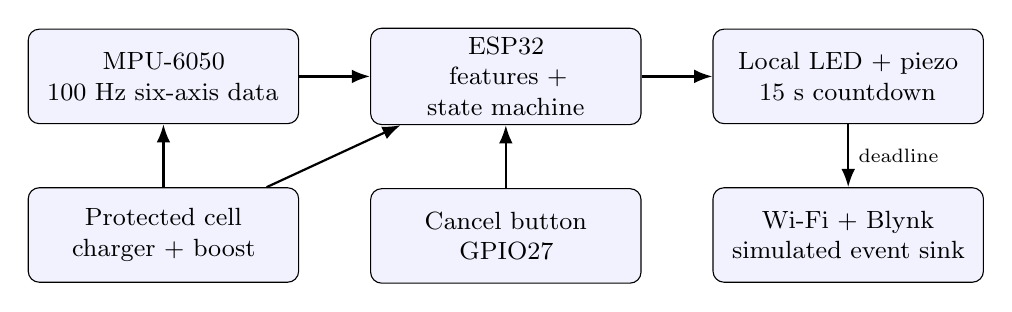
\begin{tikzpicture}[node distance=8mm and 9mm,b/.style={draw,rounded corners,fill=blue!5,align=center,font=\small,minimum height=12mm,text width=32mm},a/.style={-Latex,thick}]
\node[b](imu){MPU-6050\\100 Hz six-axis data};
\node[b,right=of imu](esp){ESP32\\features + state machine};
\node[b,right=of esp](alarm){Local LED + piezo\\15 s countdown};
\node[b,below=of imu](power){Protected cell\\charger + boost};
\node[b,below=of esp](button){Cancel button\\GPIO27};
\node[b,below=of alarm](cloud){Wi-Fi + Blynk\\simulated event sink};
\draw[a](imu)--(esp);\draw[a](esp)--(alarm);\draw[a](button)--(esp);\draw[a](power)--(imu);\draw[a](power)--(esp);\draw[a](alarm)--node[right,font=\scriptsize]{deadline}(cloud);
\end{tikzpicture}
\caption{Acquisition, local decision, user cancellation, and remote event architecture. The event sink is replaced by an instrumented service model in the execution harness.}
\end{figure}

\subsection{Circuit diagram and virtual-hardware image}
The circuit diagram details power conditioning, sensor connections, battery measurement, and warning outputs using common net labels. The resistor and capacitor values identify the operating points used in the DC interface simulation and clarify the transistor-driven piezo connection.

\begin{figure}[H]\centering\resizebox{\linewidth}{!}{\begin{circuitikz}[american,scale=.9,transform shape]
\tikzset{mod/.style={draw,rounded corners,align=center,font=\small,fill=blue!4,minimum height=10mm},lab/.style={font=\scriptsize,fill=white,inner sep=1pt}}
% Power chain, common labelled supply nets.
\node[mod,minimum width=28mm] (cell) at (1.5,12.5) {18650 cell\\2600 mAh};
\node[mod,minimum width=35mm] (charge) at (5.5,12.5) {TP4056 + DW01A\\charge / protect};
\node[mod,minimum width=28mm] (boost) at (11,12.5) {MT3608\\5 V boost};
\draw (cell.east)--(charge.west);
\draw (charge.east) to[spst] (boost.west);
\node[lab] at (8.2,13.1) {master switch};
\draw (boost.east)--(14.5,12.5) node[right,lab]{+5V};
\draw (charge.north)--++(0,.55) node[above,lab]{USB 5 V charging};
\draw (cell.south)--++(0,-.4) node[ground]{};
\draw (charge.south)--++(0,-.4) node[ground]{};
\draw (boost.south)--++(0,-.4) node[ground]{};
\node[lab,anchor=west] at (0,11.25) {All GND nets common. Master switch open during charging. VBAT = switched protected cell output.};
% Controller / sensor interface.
\node[mod,minimum width=30mm,minimum height=24mm] (imu) at (1.8,8.8) {MPU-6050\\GY-521\\0x68};
\node[mod,minimum width=32mm,minimum height=36mm] (esp) at (7.0,8.8) {ESP32\\WROOM-32};
\draw ([yshift=8mm]imu.east)--([yshift=8mm]esp.west) node[midway,lab]{VCC -- 3V3};
\draw (imu.east)--(esp.west) node[midway,lab]{SDA -- GPIO21};
\draw ([yshift=-8mm]imu.east)--([yshift=-8mm]esp.west) node[midway,lab]{SCL -- GPIO22};
\draw (imu.south)--++(0,-.4) node[ground]{};
\draw (esp.south)--++(0,-.4) node[ground]{};
\draw (esp.north)--++(0,.4) node[above,lab]{VIN = +5V};
\node[lab] at (1.8,6.9){100 nF across VCC / GND};
% Battery sensing and decoupling.
\draw (10,10.2) node[above,lab]{VBAT} to[R,l=100 k$\Omega$] (10,8.8) coordinate (adc) to[R,l=100 k$\Omega$] (10,7.2) node[ground]{};
\draw (adc)--(12,8.8) coordinate (cap) -- (13.7,8.8) node[right,lab]{GPIO34};
\draw (cap) to[C,l=100 nF] (12,7.2) node[ground]{};
\draw (14.3,10.5) node[above,lab]{+5V} to[C,l=100 $\mu$F] (14.3,9.4) node[ground]{};
% LED branch.
\node[lab,anchor=west] at (0,5.9){Local warning LED};
\draw (0.3,5.2) node[above,lab]{GPIO26} to[R,l=220 $\Omega$] (2.6,5.2) to[leD,l=red LED] (4.8,5.2) -- (5.4,5.2) node[ground]{};
% Button.
\node[lab,anchor=west] at (0,3.7){Cancel button};
\draw (0.3,2.8) node[above,lab]{GPIO27} to[push button,l=CANCEL] (3,2.8) -- (4,2.8) node[ground]{};
\node[lab,anchor=west] at (0,1.8){GPIO27 uses the ESP32 internal pull-up.};
% Piezo branch with independent supply labels.
\node[npn] (q) at (12,3.1) {};
\draw (8.1,3.1) node[above,lab]{GPIO25} to[R,l=1 k$\Omega$] (q.B);
\draw (q.E)--++(0,-.65) node[ground]{};
\draw (q.C) to[buzzer,l=5 V passive piezo] (12,5.5) -- (12,5.9) node[above,lab]{+5V};
\draw (10.8,3.1) to[R,l_=10 k$\Omega$] (10.8,1.4) node[ground]{};
\node[lab,right] at (12.5,3.1){2N2222};
\node[lab,anchor=west] at (0,.5){Supply, GPIO and ground labels identify electrically common nets. MPU-6050 signal pull-ups use 3.3 V.};
\end{circuitikz}
}
\caption{Complete connection-level circuit: power, sensing, battery divider, LED, transistor-driven piezo, and cancel input. The master switch is open during charging; the charger module provides no load-sharing function.}\end{figure}
The GY-521 uses 3.3 V power and logic. GPIO25 drives the piezo through a 2N2222 with a 1 k$\Omega$ base resistor and 10 k$\Omega$ pull-down. The battery divider has a 100 nF shunt capacitor; the 5 V rail has 100 $\mu$F decoupling. A DC sweep of 39 combinations covers 3.0--4.2 V cell voltage and 1.8, 2.0, and 2.2 V LED forward drops. It produces ADC voltages of 1.50--2.10 V, divider current of 15--21 $\mu$A, and LED current of 5.0--6.82 mA. These are executed DC interface calculations, paired with the separate time-stepped battery experiment.
The virtual-hardware image captures a specific executed confirmation state rather than an arbitrary arrangement of components. Its annotations connect the 3.610 s confirmation timestamp to the LED level, tone frequency, countdown, and converted battery input.

\fig{figures/virtual_hardware.png}{1}{Virtual-hardware image at the executed confirmation instant, 3.610 s. The rendered board and peripherals display the firmware harness state: LED high, 2400 Hz tone, and active countdown. This simulation image supplies the hardware-view evidence for the report.}

\subsection{Dataset generation and preprocessing}
The original simulation has 675 events, each ten seconds long at 100 Hz: 675,000 six-axis samples. The nine classes each contain 75 events. Normal riding, potholes, speed breakers, hard braking, sharp turning, parked tip-over, and impact with recovery are negative classes. Low-side and high-side crashes are positive classes, giving 150 positive and 525 negative events. Seed 20260828 fixes the generator; seed 20260911 supplies an additional 30 events per class, giving 270 fresh events and 270,000 samples.

Each trajectory contains roll, pitch, and yaw profiles, body-frame gravity, manoeuvre pulses, noise, bias, and clipping. Equation~\eqref{eq:gravity} expresses gravity as a three-component column vector in the body frame, using roll $\phi$ and pitch $\theta$ in radians. The normalized vector $\widehat{\mathbf g}_b$ is dimensionless; multiplication by $g_0=9.80665\,\mathrm{m\,s^{-2}}$ gives physical acceleration, while its components directly represent acceleration in units of $g$.
\begin{equation}
\label{eq:gravity}
\widehat{\mathbf g}_b=
\begin{bmatrix}
-\sin\theta\\
\sin\phi\cos\theta\\
\cos\phi\cos\theta
\end{bmatrix}\in\mathbb R^{3\times1},\qquad
\mathbf g_b=g_0\widehat{\mathbf g}_b,\qquad
\|\widehat{\mathbf g}_b\|_2=1.
\end{equation}

Here the subscript $b$ denotes the sensor body frame and the entries are ordered along its $x$, $y$, and $z$ axes. The symbols $\phi$ and $\theta$ are roll and pitch angles in radians; the trigonometric functions therefore take radian arguments. A hat denotes normalization: $\widehat{\mathbf g}_b$ is a dimensionless $3\times1$ column vector, whereas $\mathbf g_b$ is the physical gravity contribution in m/s$^2$. The notation $\mathbb R^{3\times1}$ specifies three real-valued components, and $\|\cdot\|_2$ denotes the Euclidean norm. The scalar $g_0=9.80665$ m/s$^2$ is standard gravitational acceleration, not a fitted parameter; the constant 1 specifies unit vector length. At $\phi=\theta=0$, the normalized vector is $[0,0,1]^{\mathsf T}$. In this convention positive roll produces a positive $y$ component and positive pitch a negative $x$ component. Yaw does not enter this gravity projection because rotation about the vertical reference does not change gravity.

Linear pulses are added to this gravity vector. The generator constructs angular channels from numerical derivatives of the three angle trajectories, expressed in degrees per second. This Euler-angle derivative construction is a prescribed signal model; coupling between Euler derivatives and rigid-body angular velocity is a model-fidelity limitation for large simultaneous rotations.

Event time is uniformly drawn from 3.8--5.2 s. Acceleration bias has standard deviation 0.018 $g$ and sample noise 0.022 $g$; angular-rate bias has standard deviation 0.8 $\degree$/s and sample noise 1.5 $\degree$/s. Samples are clipped to the configured full-scale ranges. Low-side final roll spans 48--105$\degree$, while high-side roll spans 70--135$\degree$. The low-side distribution deliberately includes final angles below the detector's 55$\degree$ gate. High-side impact pulses span 3.0--11.5 $g$ and low-side pulses span 0.8--5.5 $g$ before vector addition and clipping.

For external signal analysis, seven critical manoeuvres and four fall recordings are loaded from the published PTW supplement~\cite{boubezoul2019dataset}. Finite numeric rows are retained, six channels are anti-alias filtered and resampled from 1 kHz to 100 Hz using polyphase resampling with a Kaiser window, acceleration is converted from m/s$^2$ to $g$ using 9.80665, and angular rate remains in degrees per second. The four fall windows are centred at 40.132, 34.288, 35.876, and 43.486 s, respectively, with a $\pm1.5$ s interval. Whole manoeuvre recordings supply the negative gate comparison. These three-second fall windows evaluate individual gates; they are distinct from the full rest-and-countdown evaluation.

\subsection{Data split and evaluation protocol}
The original events are partitioned within each scenario by generation order: the first 45 form the development partition, the next 15 the validation partition, and the final 15 the test partition. This yields 405/135/135 events, or 60/20/20\%. Whole events remain in one partition; adjacent samples are never split across partitions. \texttt{results/splits.csv} lists every assignment.

CrashGuard is a fixed rule system, so no model weights are fitted. The partitioned results are a retrospective breakdown of the existing replay. The fresh 270-event set is generated after freezing the detector for this study and evaluated without selecting thresholds from its outcomes. It provides a separate random-stream test within the same scenario family. Public PTW recordings are reserved for the external gate analysis, and human-fall datasets are used for literature context rather than motorcycle labels.

\subsection{Features, calibration, and decision equations}
Startup calibration averages 200 stationary samples. A gravity norm outside 0.85--1.15 $g$ or gyro RMS above 5 $\degree$/s causes a retry. The accepted acceleration vector becomes the reference gravity, and the three gyro means become bias offsets. Let $\mathbf a=[a_x,a_y,a_z]^{\mathsf T}$ and $\mathbf r=[r_x,r_y,r_z]^{\mathsf T}$ denote acceleration and reference-gravity column vectors, with components expressed numerically in $g$; let $\boldsymbol\omega=[\omega_x,\omega_y,\omega_z]^{\mathsf T}$ contain angular rates in degrees per second. Equation~\eqref{eq:accel} reduces the acceleration vector to a scalar Euclidean magnitude. The detector compares this numerical magnitude with thresholds such as 2.0 and 0.35, corresponding to physical magnitudes of $2g$ and $0.35g$.
\begin{equation}\label{eq:accel}
A=\|\mathbf a\|_2=\sqrt{a_x^2+a_y^2+a_z^2}.
\end{equation}

In Equation~\eqref{eq:accel}, $a_x$, $a_y$, and $a_z$ are the simultaneously sampled acceleration components divided by $g_0$; they are numerical values expressed in $g$ units rather than SI acceleration values. Their collection $\mathbf a$ is a column vector, and $A$ is its nonnegative scalar magnitude. Thus $A=1$ corresponds to a physical magnitude of one $g$, while $A=2.0$ corresponds to two $g$. The exponent 2 squares each component and the square root restores the magnitude scale. For the configured $\pm16g$ sensor range, the raw signed acceleration counts are divided by 2048 counts per $g$ in the firmware. Event processing samples these components every 10 ms, equivalent to 100 Hz.


Equation~\eqref{eq:rotation} combines the three angular-rate components into one nonnegative rotational magnitude. This scalar has units of degrees per second and is compared with the correlation and final-rest limits. Taking its norm makes the gate insensitive to which sensor axis contains the dominant rotation.
\begin{equation}\label{eq:rotation}
\Omega=\|\boldsymbol\omega\|_2=\sqrt{\omega_x^2+\omega_y^2+\omega_z^2}.
\end{equation}

Here $\omega_x$, $\omega_y$, and $\omega_z$ are the bias-corrected angular rates about the sensor axes, each in degrees per second; $\boldsymbol\omega$ is their $3\times1$ column vector. The scalar $\Omega$ is the Euclidean norm and has the same degrees-per-second unit. A negative component indicates rotation in the opposite axis direction, but squaring removes that sign in the magnitude. The configured $\pm2000\degree$/s raw gyro values are divided by 16.4 counts per degree per second, then their stationary means are subtracted. The detector compares $\Omega$ with 90$\degree$/s for rotational corroboration and 30$\degree$/s for final-rest acceptance; these are configuration thresholds, not factors in the norm formula.


Equation~\eqref{eq:tilt} computes the angle between the current acceleration vector and the calibrated reference vector. The transposed product is a scalar dot product, division by both norms produces a dimensionless cosine, and clipping protects the inverse cosine against round-off. The factor $180/\pi$ converts the returned angle to degrees.
\begin{equation}\label{eq:tilt}
\Theta=\frac{180}{\pi}\arccos\!\left[\operatorname{clip}\left(\frac{\mathbf a^{\mathsf T}\mathbf r}{\|\mathbf a\|_2\|\mathbf r\|_2},-1,1\right)\right].
\end{equation}

In this equation $\Theta$ is the scalar angle in degrees, constrained to $[0,180]$ for a valid nonzero input. The current normalized acceleration vector is $\mathbf a$ and the stationary reference is $\mathbf r$, whose components are the means of 200 accepted calibration samples in the same $g$ convention. The superscript $\mathsf T$ denotes transpose, so $\mathbf a^{\mathsf T}\mathbf r$ is the scalar sum $a_xr_x+a_yr_y+a_zr_z$. Dividing by the two Euclidean norms forms a dimensionless cosine. For a scalar input $u$, $\operatorname{clip}(u,-1,1)$ means $\min(1,\max(-1,u))$; the bounds $-1$ and $1$ are the valid inverse-cosine domain. The function $\arccos$ returns radians, and $180/\pi$ converts them to degrees, with $\pi\approx3.141592653589793$. The numerical tolerance $10^{-6}$ applies to the product of the normalized vector norms and prevents division by a near-zero denominator.

When the denominator is below $10^{-6}$, the implementation returns zero tilt. Tilt is derived from the instantaneous acceleration vector; it is most interpretable during the near-gravity rest interval.

Ride activity is present when $|A-1|\geq0.08$ or $\Omega\geq4\degree$/s. Activity evidence accumulates toward 1000 ms and decays at half rate during inactivity. The implementation refreshes a 5000 ms active-riding deadline while evidence is full. Once qualified, a candidate starts on $A\geq2.0$ or $A\leq0.35$. Rotation at or above 90$\degree$/s is correlated with the candidate using a 750 ms interval. Equation~\eqref{eq:rest} defines the Boolean final-rest predicate from three simultaneous scalar comparisons. It requires a large tilt, near-gravity acceleration, and low angular motion; $A$ is the numerical magnitude in $g$ units, while the angular limits retain their explicit units. Holding this predicate continuously establishes the intended post-event rest evidence:
\begin{equation}
 \label{eq:rest} R=(\Theta\geq55\degree)\land(0.70\leq A\leq1.30)\land(\Omega\leq30\degree/\mathrm{s}).
\end{equation}

The variable $R$ is Boolean: it is true only when every condition joined by $\land$ (logical AND) is true; otherwise it is false. The measured inputs are $\Theta$ in degrees, numerical acceleration magnitude $A$ in $g$ units, and $\Omega$ in degrees per second. The constants 55$\degree$, 0.70, 1.30, and 30$\degree$/s are, respectively, the minimum tilt, lower near-gravity bound, upper near-gravity bound, and maximum rotational motion allowed at rest. The acceleration interval corresponds to $1g\pm0.30g$. The inclusive comparisons accept values exactly at their limits. The 2000 ms rest hold and 6000 ms candidate timeout are separate time constants enforced by the state machine; they are not encoded by the instantaneous predicate itself.

Holding $R$ for 2000 ms confirms a crash; verification times out after 6000 ms. Confirmation starts the alarm and 15,000 ms cancel window. The finite-state implementation has constant memory and constant work per sample.

\subsection{Algorithm and flowchart}
The algorithm table presents the implemented procedure in execution order, including calibration, scheduled acquisition, cancellation, and the final event operation. It also identifies where a sensor or network failure changes the normal control path.

\begin{table}[H]\centering\small\caption{Algorithm 1: Ordered firmware procedure from sensor initialization to one-shot incident submission. Each row identifies an operation in the implemented control path, including its timing or failure branch. Acquisition is scheduled every 10 ms (100 Hz); stationary calibration uses 200 samples; a confirmed event activates the LED and 2400 Hz piezo command before a 15 s cancellation interval. A sensor-read error skips the detector update, and the deadline operation records the service outcome without implying user notification receipt.}
\begin{tabularx}{\linewidth}{@{}rX@{}}\toprule
Step & Operation\\\midrule
1 & Configure GPIO and MPU-6050; stop safely if the sensor probe fails.\\
2 & Collect 200 samples; reject moving/invalid calibration and retry until a valid reference is obtained.\\
3 & Begin asynchronous Wi-Fi association and initialize the 10 ms sample schedule.\\
4 & Check the cancel-button edge; cancel a countdown or acknowledge an alert and silence local outputs.\\
5 & At each sample deadline, read the 14-byte sensor burst. Log and skip the detector update on failure.\\
6 & Compute $A$, $\Omega$, and $\Theta$; update activity evidence and candidate/rotation/rest state.\\
7 & On confirmation, set LED high, start the 2400 Hz tone, and store the countdown start time.\\
8 & At elapsed countdown $\geq15$ s, issue one event operation; record submitted, disabled, Wi-Fi unavailable, or cloud unavailable.\\
9 & Keep the local warning active until rider acknowledgement; repeat acquisition.\\\bottomrule
\end{tabularx}\end{table}

The flowchart emphasizes the temporal order of the decision and the two principal return paths. Rejection resumes acquisition, while rider cancellation interrupts the pending warning before an event operation becomes due.

\begin{figure}[H]\centering
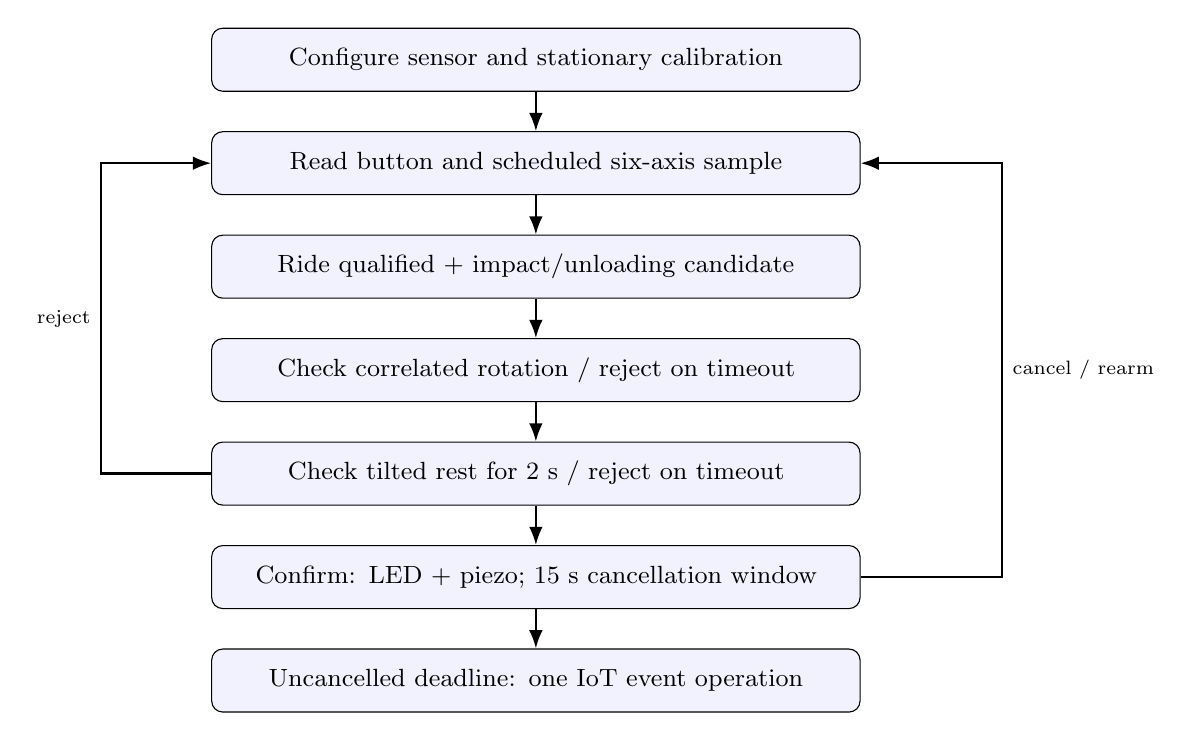
\begin{tikzpicture}[node distance=5mm,b/.style={draw,rounded corners,fill=blue!5,align=center,text width=80mm,minimum height=8mm,font=\small},a/.style={-Latex,thick}]
\node[b](start){Configure sensor and stationary calibration};
\node[b,below=of start](sample){Read button and scheduled six-axis sample};
\node[b,below=of sample](ride){Ride qualified + impact/unloading candidate};
\node[b,below=of ride](rot){Check correlated rotation / reject on timeout};
\node[b,below=of rot](rest){Check tilted rest for 2 s / reject on timeout};
\node[b,below=of rest](count){Confirm: LED + piezo; 15 s cancellation window};
\node[b,below=of count](event){Uncancelled deadline: one IoT event operation};
\foreach \a/\b in {start/sample,sample/ride,ride/rot,rot/rest,rest/count,count/event}\draw[a](\a)--(\b);
\draw[a](count.east)--++(18mm,0)|-node[pos=.25,right,font=\scriptsize]{cancel / rearm}(sample.east);
\draw[a](rest.west)--++(-14mm,0)|-node[pos=.25,left,font=\scriptsize]{reject}(sample.west);
\end{tikzpicture}\caption{Flowchart of successful detection and the cancellation/rejection return paths. Sensor-read errors return to the scheduled acquisition loop.}
\end{figure}

\subsection{Baselines and metrics}
The acceleration-only baseline fires when $A\geq2.0$. The strict ordered comparison requires $A\geq4.0$, then $\Omega\geq200\degree$/s within 500 ms, then tilt at least 60$\degree$ with acceleration in 0.70--1.30 $g$ for three seconds; its overall verification limit is eight seconds. These are executable comparison rules, not reproductions of the cited learned models.

Let $TP$, $TN$, $FP$, and $FN$ denote true positives, true negatives, false positives, and false negatives, respectively. All metric denominators below are positive in the reported experiments.

Accuracy summarizes the fraction of correct decisions across all events. Its denominator includes both classes, so a high value can coexist with poor sensitivity when negative events are more numerous.
\begin{equation}\label{eq:accuracy} \mathrm{Accuracy}=\frac{TP+TN}{TP+TN+FP+FN}.\end{equation}

For Equation~\eqref{eq:accuracy}, $TP$ counts true crash events classified as crash, $TN$ counts true non-crash events classified as non-crash, $FP$ counts non-crash events classified as crash, and $FN$ counts crash events classified as non-crash. All four quantities are nonnegative integer event counts. Their sum is the evaluation-set size $N$: $N=675$ for the primary set and $N=270$ for the fresh set. The numerator counts correct decisions across both classes. Accuracy is a dimensionless fraction in $[0,1]$ and is multiplied by 100 when reported as a percentage; it is defined only when $N>0$.


Sensitivity measures the fraction of positive events detected. It directly exposes missed crashes and is therefore reported alongside accuracy and broken down by low-side and high-side scenario.
\begin{equation}\label{eq:sensitivity} \mathrm{Sensitivity}=\frac{TP}{TP+FN}.\end{equation}

Here $TP$ is the number of correctly detected crash events and $FN$ is the number of missed crash events. The denominator $TP+FN$ is the number of labelled positives: 150 in the primary simulation and 60 in the fresh simulation. Sensitivity is also called recall or the true-positive rate. It has no physical unit, lies in $[0,1]$, and is multiplied by 100 for percentage reporting. Its denominator must be nonzero. For the fresh CrashGuard result, the substitution is $43/(43+17)=0.7167$, giving 71.7\% after rounding.


Specificity measures the fraction of negative events correctly rejected. It describes nuisance-alarm control within the evaluated negative set and must be interpreted with the number and diversity of those events.
\begin{equation}\label{eq:specificity} \mathrm{Specificity}=\frac{TN}{TN+FP}.\end{equation}

In Equation~\eqref{eq:specificity}, $TN$ counts correctly rejected non-crash events and $FP$ counts non-crash events that trigger a false detection. Their sum is the negative-event denominator: 525 in the primary simulation and 210 in the fresh simulation. Specificity is a dimensionless fraction between zero and one, reported in percent after multiplication by 100, and requires at least one labelled negative. For the fresh CrashGuard result, $TN=210$ and $FP=0$, so the observed fraction is 1. This finite-sample observation is accompanied by a Wilson interval rather than interpreted as universal perfect rejection.


Precision measures the proportion of predicted positives that are true positives. It characterizes the reliability of an emitted event within the test distribution and can change when event prevalence changes.
\begin{equation}\label{eq:precision} \mathrm{Precision}=\frac{TP}{TP+FP}.\end{equation}

Here $TP$ is the count of correctly classified crash events and $FP$ the count of false crash detections. The denominator $TP+FP$ counts all events predicted positive, irrespective of their true class. Precision is dimensionless on $[0,1]$ and describes the positive predictions under the test-set event prevalence. If no positive event is predicted, the mathematical ratio has a zero denominator; the evaluation code assigns zero precision for that case. Every reported detector predicts at least one positive event, so this fallback does not affect the presented values. CrashGuard has fresh-set precision $43/(43+0)=1$.


The F1-score combines precision and sensitivity into one count-based statistic. It penalizes both false positives and false negatives and complements specificity without replacing the separate confusion counts.
\begin{equation}\label{eq:f1} F_1=\frac{2TP}{2TP+FP+FN}.\end{equation}

In this expression $TP$, $FP$, and $FN$ are event counts as defined above. The constant factor 2 weights the correctly detected positives in the count form of the harmonic mean of precision and sensitivity; the subscript 1 indicates equal precision and recall weighting. F1 is dimensionless and reported as a decimal between zero and one, unlike the percentage columns for accuracy, sensitivity, and specificity. The denominator must be positive. For the fresh CrashGuard counts, $2(43)/[2(43)+0+17]=86/103=0.83495$, rounded to 0.835.


The false-positive rate measures the fraction of negative events that trigger incorrectly. It equals one minus specificity and supports a direct comparison of nuisance alarms between the three rules on identical events.
\begin{equation}\label{eq:fpr} \mathrm{FPR}=\frac{FP}{TN+FP}.\end{equation}

The abbreviation FPR denotes false-positive rate. The numerator $FP$ counts negative events incorrectly predicted positive, and the denominator $TN+FP$ counts all labelled negatives. The rate is dimensionless, lies in $[0,1]$, and equals one minus specificity when the negative denominator is nonzero. Multiplication by 100 converts it to percent. For the fresh acceleration-only baseline, $FP=108$ and $TN=102$, giving $108/210=0.5143$, or 51.4\%; for CrashGuard the corresponding numerator is zero. This event-level rate is distinct from false alarms per riding hour, which would require an exposure-time denominator.


Delay is confirmation time minus the start of the candidate that reaches confirmation. It is computed only for detected positive events. The acceleration-only method has zero additional confirmation hold by definition. For a binomial proportion $\hat p=x/n$, the Wilson equation gives lower and upper confidence bounds from the observed success count $x$ and sample count $n$. Using $z=1.959964$ gives a 95\% interval that remains informative when all observed negatives are rejected. Sensitivity and specificity use their respective positive and negative denominators~\cite{wilson1927interval}:
\begin{equation}\label{eq:wilson}
\begin{aligned}
p_{\mathrm L}&=\frac{\hat p+z^2/(2n)-z\sqrt{\hat p(1-\hat p)/n+z^2/(4n^2)}}{1+z^2/n},\\[2mm]
p_{\mathrm U}&=\frac{\hat p+z^2/(2n)+z\sqrt{\hat p(1-\hat p)/n+z^2/(4n^2)}}{1+z^2/n}.
\end{aligned}
\end{equation}
In Equation~\eqref{eq:wilson}, $p_{\mathrm L}$ and $p_{\mathrm U}$ are the lower and upper limits for the relevant success probability $p$. The first expression subtracts the uncertainty term to obtain the lower limit; the second adds it to obtain the upper limit. Together they define the interval $[p_{\mathrm L},p_{\mathrm U}]$. The integer $x$ is the observed number of successes, $n>0$ is the number of eligible events, and $\hat p=x/n$ is the estimated success proportion. For sensitivity, $x=TP$ and $n=TP+FN$; for specificity, $x=TN$ and $n=TN+FP$. The dimensionless constant $z=1.959963984540054$ is the 97.5th percentile of the standard normal distribution, producing the two-sided 95\% interval; 1.959964 is its rounded presentation. The constants 2 and 4 arise from the Wilson score construction and are not tuned detector settings. All proportions and bounds are dimensionless and become percentages after multiplication by 100. These intervals characterize finite counts within the generated event distribution and do not remove model-domain dependence.

\section{Experimental Results and Discussion}
\subsection{Experimental conditions}
C++17 executables are compiled with optimization and strict warning flags. Python, NumPy, SciPy, and Matplotlib generate data, replay the detector, calculate metrics, and render plots. All events start with a fresh detector. The firmware peripheral harness uses a virtual clock, a 14-byte register buffer, instrumented GPIO/tone outputs, and a local Blynk-compatible sink. It invokes the unchanged firmware code with controlled returns for probe failure, truncated reads, link failure, and cloud timeout. No network credentials are required for these simulations.

The original 675-event pipeline was re-executed and reproduced its confusion counts. The fresh-seed experiment adds 270 events. Across both motion datasets, 945 events and 945,000 samples were processed. Fourteen harness scenarios and 39 DC combinations supplement nine battery-discharge cases. The experiments exercise different layers and their counts are reported separately.

\subsection{Original and fresh performance comparison}
The reproduced comparison below places all three decision rules on the same 675 original events. Confusion counts expose the origin of each score: CrashGuard improves nuisance-alarm rejection over acceleration-only detection, while the strict ordered rule loses substantially more positive events.

\begin{table}[H]\centering\small\caption{Event-level comparison of three executable detection rules on the same 675-event simulation (seed 20260828; 150 crash events and 525 non-crash events). TP, TN, FP, and FN denote true positives, true negatives, false positives, and false negatives, respectively, and are event counts. Acc., Sens., and Spec. are accuracy, sensitivity, and specificity in percent; F1 is dimensionless on $[0,1]$. Each row is one detector, so differences reflect rule behavior on identical inputs rather than differences in data composition.}
\resizebox{\linewidth}{!}{\begin{tabular}{@{}lrrrrrrrr@{}}\toprule
Detector & TP & TN & FP & FN & Acc. & Sens. & Spec. & F1\\\midrule
Acceleration-only & 134 & 236 & 289 & 16 & 54.8 & 89.3 & 45.0 & 0.468\\
Strict ordered & 39 & 525 & 0 & 111 & 83.6 & 26.0 & 100.0 & 0.413\\
CrashGuard & 114 & 525 & 0 & 36 & 94.7 & 76.0 & 100.0 & 0.864\\\bottomrule
\end{tabular}}\end{table}
The next table evaluates the same frozen rules on 270 newly generated events. This separate random stream checks whether the earlier specificity advantage persists and reveals the remaining sensitivity cost without selecting thresholds from these results.

\begin{table}[H]\centering\small\caption{Independent-random-stream evaluation of the unchanged rules on 270 generated events (seed 20260911; 60 crash and 210 non-crash events). TP/TN/FP/FN are event-level confusion counts; Acc., Sens., and Spec. are accuracy, sensitivity, and specificity in percent; F1 is a dimensionless precision--recall score. No threshold is selected using this set. The comparison tests repeatability within the same signal-generator family: it is not a vehicle-wise or road-session-wise external validation.}
\resizebox{\linewidth}{!}{\begin{tabular}{@{}lrrrrrrrr@{}}\toprule Detector & TP & TN & FP & FN & Acc. & Sens. & Spec. & F1\\\midrule
Acceleration-only & 52 & 102 & 108 & 8 & 57.0 & 86.7 & 48.6 & 0.473 \\
Strict ordered-threshold & 13 & 210 & 0 & 47 & 82.6 & 21.7 & 100.0 & 0.356 \\
CrashGuard & 43 & 210 & 0 & 17 & 93.7 & 71.7 & 100.0 & 0.835 \\
\bottomrule\end{tabular}}\end{table}
On the original replay, CrashGuard removes 289 false positives relative to acceleration-only detection but introduces 20 additional misses. On the fresh set, it removes 108 false positives while introducing nine additional misses. This is a specificity--sensitivity tradeoff. The strict ordered rule is also specific but detects only 13 of 60 fresh positive events. CrashGuard detects 43, a gain of 30 events on that same set.

Fresh-set sensitivity is 71.7\% with a 95\% Wilson interval of 59.2--81.5\%. Observed specificity is 100.0\% with an interval of 98.2--100.0\%. The original sensitivity interval is 68.6--82.1\%, and specificity interval is 99.3--100.0\%. Zero observed false positives therefore describes the finite negative sets. It does not imply perfect specificity across all riding conditions.

The partition table reports whole-event counts and confusion outcomes for each data subset. It distinguishes the retrospective development/validation/test breakdown from the fresh-seed experiment, preventing those two evaluation roles from being conflated.

\begin{table}[H]\centering\small\caption{CrashGuard confusion counts and F1-score by whole-event data partition. The original simulation is split within each of nine scenarios into 45 development, 15 validation, and 15 retrospective-test events, giving 405/135/135 events overall. The fresh-seed set contains 30 additional events per scenario. TP/TN/FP/FN are event counts and sum to the Events column; F1 is dimensionless. These are fixed-rule evaluations, with no learned weights fitted in any partition.}
\begin{tabular}{@{}lrrrrrr@{}}\toprule
Partition & Events & TP & TN & FP & FN & F1\\\midrule
Development & 405 & 67 & 315 & 0 & 23 & 0.854\\
Validation & 135 & 23 & 105 & 0 & 7 & 0.868\\
Retrospective test & 135 & 24 & 105 & 0 & 6 & 0.889\\
Fresh-seed test & 270 & 43 & 210 & 0 & 17 & 0.835\\\bottomrule
\end{tabular}\end{table}

\subsection{Scenario analysis and graphs}
All seven negative classes are rejected in both simulation sets. All 75 original high-side events and all 30 fresh high-side events are detected. Low-side detection is 39/75 in the original set and 13/30 in the fresh set. Consequently, all 36 original misses and all 17 fresh misses belong to the low-side class. These profiles include weaker impacts, slower motion, and smaller final lean than the high-side generator. The fixed gates select a narrower subset of that distribution.
The scenario plot separates correct decisions by motion class for the original and fresh datasets. Its main finding is that aggregate accuracy masks a concentrated low-side failure mode, while high-side events and all seven negative classes retain complete correctness in these finite sets.

\fig{figures/scenarios.pdf}{1}{Per-scenario event correctness from the executed original and fresh-seed simulations. Each original class contains 75 events; each fresh class contains 30.}
The signal-profile figure shows how magnitude, angular rate, and tilt evolve across representative generated events. A transient pothole and an unqualified parked tip-over differ from a correlated fall-like sequence, illustrating why the same peak amplitude need not produce the same state transition.

\fig{figures/simulated_profiles.pdf}{.95}{Generated six-axis event profiles transformed into acceleration, rotation, and tilt features. The curves illustrate why an isolated impact, a parked tip-over, and a crash-like sequence receive different decisions.}
The paired plots connect fresh-set classification errors with confirmation timing. The confusion matrix includes all 270 events, whereas the delay histogram includes only the 43 detected positives; this difference in denominators is essential when interpreting latency.

\fig{figures/confusion_delay.pdf}{1}{Fresh-test confusion counts and candidate-to-confirmation delays. The delay histogram includes the 43 detected positives; missed events remain represented in the confusion matrix.}

\subsection{External public-data gate analysis}
The public-data table summarizes the four fall windows after unit conversion and resampling. Peak and minimum acceleration explain unloading-gate activation, while peak angular rate explains the rotation gate; the final column records independent gate crossings rather than a complete crash decision.

\begin{table}[H]\centering\small\caption{Inertial signal extrema in four public powered-two-wheeler (PTW) fall windows after anti-aliased resampling from 1 kHz to 100 Hz. Each row summarizes a 3 s interval centered on the specified event time. Peak and minimum $A$ are acceleration-magnitude values in $g$ units; peak $\Omega$ is angular-rate magnitude in degrees per second. ``Both gates'' means that the acceleration condition ($A\geq2.0$ or $A\leq0.35$) and rotation condition ($\Omega\geq90\degree$/s) each occur somewhere in that window; their temporal correlation and final-rest condition are not implied.}
\begin{tabularx}{\linewidth}{@{}Xrrrr@{}}\toprule
Fall recording & Peak $A$ ($g$) & Min. $A$ ($g$) & Peak $\Omega$ ($\degree$/s) & Both gates\\\midrule
Slippery straight road & 1.169 & 0.013 & 179.4 & Yes\\
Leaning motorcycle & 1.878 & 0.041 & 144.1 & Yes\\
Roundabout & 1.690 & 0.011 & 150.5 & Yes\\
Curve & 1.436 & 0.130 & 151.6 & Yes\\\bottomrule
\end{tabularx}\end{table}
All four fall windows cross CrashGuard's unloading and rotation gates, while none reaches the strict 4 $g$ and 200$\degree$/s gates. Three of seven critical manoeuvres also cross both CrashGuard gates somewhere in their recordings. This demonstrates that amplitude gates alone do not separate all positive and negative examples. Their independent crossings do not establish temporal correlation, qualified riding, or final rest. The full recording features and all seven manoeuvre names are retained in \texttt{external\_ptw\_features.csv}.

\subsection{Timing, cancellation, and IoT communication}
The original median candidate-to-confirmation delay is 2.31 s; the fresh median is 2.33 s. The strict ordered baseline requires 3.12 s median additional confirmation time in both sets. The temporal hold therefore accounts for a substantial part of decision latency. Adding the intentional 15 s cancellation interval yields 17.33 s from candidate to event deadline at the fresh-set median, before any service connection delay.

In the raw-register harness, riding is qualified before a rotation at 1500 ms and an impact at 1600 ms. Tilted rest begins at 1610 ms, confirmation occurs at 3610 ms, and the event becomes due at 18,610 ms. The test verifies that the state remains \texttt{COUNTDOWN} at 18,600 ms and becomes \texttt{ALERT\_DUE} ten milliseconds later. GPIO26 is high and the tone frequency is 2400 Hz after confirmation. The simulated service receives exactly one \texttt{crash\_confirmed} event with a 143-byte description.

A separate cancellation test presses GPIO27 at 4010 ms. The local outputs become inactive and the detector remains idle through 20,000 ms. The event path distinguishes a submission to the instrumented service, disabled configuration, Wi-Fi failure, and cloud failure. A description names acceleration, angular rate, and tilt at confirmation, and explicitly reports that a location fix is unavailable. The tested device has no GNSS input. Blynk event identity and payload formation follow the platform's firmware event interface~\cite{blynkevents}.

The virtual-hardware image and state traces provide a replay dashboard: acquisition values, countdown state, alarm outputs, and event outcome are tied to one execution. A deployed application can present the same fields through a Blynk device template. Continuous virtual-pin telemetry is a separate extension; the evaluated sketch's remote operation is the event submission.

\subsection{Test cases, expected versus actual results, and fault handling}
\small
The firmware test table pairs each injected condition with its intended response and actual trace. Conformance cases verify specified behavior, while fault-characterization cases preserve evidence of unmet continuity or recovery criteria even when the regression assertion itself succeeds.

\begin{longtable}{@{}>{\raggedright\arraybackslash}p{.05\linewidth}>{\raggedright\arraybackslash}p{.20\linewidth}>{\raggedright\arraybackslash}p{.29\linewidth}>{\raggedright\arraybackslash}p{.35\linewidth}@{}}
\caption{Fourteen exact-firmware experiments with deterministic sensor, GPIO, clock, and service models. ID identifies the case; Stimulus specifies the injected input or failure; Expected behavior / criterion states the control requirement; Actual result records the observed trace and interpretation. All reported times are virtual-clock milliseconds unless seconds are explicitly written. Alarm 1/0 means the local warning is commanded active/inactive. T9, T11, and T13 characterize continuity, blocking, and recovery weaknesses; a passing regression assertion reproduces these observations and does not certify fault tolerance.}\label{tab:tests}\\
\toprule ID & Stimulus & Expected behavior / criterion & Actual result and interpretation\\\midrule\endfirsthead
\toprule ID & Stimulus & Expected behavior / criterion & Actual result and interpretation\\\midrule\endhead
T1 & Sensor absent at boot & Probe failure; safe stop; alarm off & Fatal marker and safe-stop loop observed; alarm 0. Conforms.\\
T2 & Ten-byte sensor burst & Reject incomplete 14-byte read & Warning emitted; state remains IDLE. Conforms.\\
T3 & I\textsuperscript{2}C error status & Skip invalid sample & Warning emitted; state remains IDLE. Conforms.\\
T4 & 100$\degree$/s during calibration & Reject motion above 5$\degree$/s RMS & Calibration rejected. Conforms.\\
T5 & Stationary gravity input & Accept 200 valid samples & Calibration accepted after 200 samples. Conforms.\\
T6 & ADC returns 1850 mV & Reconstruct cell voltage with factor two & 3.700 V returned. Conforms.\\
T7 & Cancel at 4010 ms & Silence outputs and suppress deadline & Alarm 0; IDLE through 20 s. Conforms.\\
T8 & Uncancelled crash & 15,000 ms from confirmation to one event & 3610 ms confirmation; 18,610 ms deadline; one event. Conforms.\\
T9 & Missing reads during rest & Desired: require continuous valid rest evidence & Confirmation at 3610 ms despite a sample gap. Continuity defect exposed.\\
T10 & Wi-Fi unavailable at deadline & Explicit skip and local alarm retained & Zero sink events; Wi-Fi skip marker; alarm 1. Conforms.\\
T11 & Cloud connection fails & Explicit failure; characterize blocking & Zero sink events; 5000 ms blocking; alarm 1. Blocking risk exposed.\\
T12 & Connected simulated sink & Correct event code and bounded payload & One event; code \texttt{crash\_confirmed}; 143 bytes. Conforms.\\
T13 & Wi-Fi recovers after deadline & Desired: eventual incident delivery & Zero events after recovery. Missing retry exposed.\\
T14 & Credential-free build & Disabled marker and local alarm retained & Not-configured marker; alarm 1. Conforms.\\\bottomrule
\end{longtable}
\normalsize
All fourteen executable assertions complete successfully. For T9 and T13, the assertions reproduce the observed deficiencies; their desired system-level criteria are unmet. This distinction prevents regression reproducibility from being mistaken for a successful safety response.

Sensor failure at startup enters a fatal stop rather than allowing uninitialized values into the detector. Short reads and bus errors skip the detector update. However, rest timing uses elapsed timestamps, so failed reads can bridge an otherwise continuous-rest interval: T9 provides valid rest at 1610 ms, failed reads at 2000 and 3000 ms, then valid rest at 3610 ms. The detector confirms. A future implementation should reset accumulated rest evidence when sensor freshness exceeds a bounded gap.

Network failure preserves the local warning and produces an explicit reason. During cloud connection failure, the configured 5000 ms connection timeout advances the virtual clock and blocks the current firmware call. The next acquisition can report a missed deadline. After the event becomes due, the state remains latched and the current implementation performs no automatic replay of a skipped event. T13 demonstrates that restoring Wi-Fi does not deliver that incident. Persistent queuing and cooperative connection management directly address these measured control-flow outcomes.

The successful GPIO/tone assertions characterize commanded outputs. A disconnected piezo or failed LED cannot be diagnosed from the present firmware because it has no actuator feedback input. The circuit and alarm model therefore expose command state, while physical output integrity is an additional sensing problem for future work.

\subsection{Expected performance versus actual performance}
The objective-to-result table brings classifier performance, warning timing, recovery, and endurance into a common assessment. Each row connects a design aim to an executed observation and states the engineering implication, including objectives that require further improvement.

\begin{table}[H]\centering\small\caption{System-level acceptance objectives, corresponding experimental observations, and engineering interpretation. The classification rows report successful decisions or false alarms divided by the relevant event count in the original and fresh simulations. Timing rows use the deterministic firmware clock; the recovery rows report whether valid-rest evidence and eventual event delivery satisfy their intended criteria. The endurance row refers specifically to the 120 mA, 5 V load and 90\% converter-efficiency simulation. Meeting one row does not establish that the remaining classification, recovery, and power objectives are met.}
\begin{tabularx}{\linewidth}{@{}>{\raggedright\arraybackslash}p{.26\linewidth}>{\raggedright\arraybackslash}p{.36\linewidth}X@{}}\toprule
Objective & Actual experiment & Interpretation\\\midrule
Reject road disturbances & 0/525 original and 0/210 fresh negative false alarms & Achieved within both scenario sets.\\
Detect crash-like events & 114/150 original; 43/60 fresh & Low-side sensitivity remains the main classification weakness.\\
Provide cancellation & Alarm silenced at 4010 ms; IDLE through 20 s & User cancellation conforms.\\
Enforce 15 s alert interval & 18,610 minus 3610 = 15,000 ms & Exact virtual-clock deadline achieved.\\
Maintain valid rest evidence & Sensor gap spans rest timer & Freshness reset required.\\
Recover event delivery & Zero events after link restoration & Persistent retry required.\\
Support a 12 h nominal operating case & 12.64 h at 120 mA and 90\% efficiency & Nominal simulated case exceeds 12 h; other loads can fall below it.\\\bottomrule
\end{tabularx}\end{table}

\subsection{Power simulation}
The battery simulation uses a finite usable-charge reservoir rather than a fixed operating-time input. Equation~\eqref{eq:charge_initial} calculates its initial charge from the nominal capacity and the usable-capacity fraction. Here $C_{\mathrm{nom}}=2.6$ Ah (2600 mAh) is nominal cell capacity, $f_{\mathrm{use}}=0.90$ is the dimensionless fraction made available to the model, and $q_0$ is the initial usable charge in ampere-hours. The subscript 0 denotes the start of discharge. Both inputs are prescribed simulation parameters, and the multiplication gives $q_0=2.34$ Ah.
\begin{equation}\label{eq:charge_initial}
q_0=C_{\mathrm{nom}}f_{\mathrm{use}}=(2.6\,\mathrm{Ah})(0.90)=2.34\,\mathrm{Ah}.
\end{equation}

Equation~\eqref{eq:cell_voltage} defines the linear voltage profile used during discharge. The variable $q$ is remaining usable charge in Ah and satisfies $0\leq q\leq q_0$ while the model is evaluated. The function $V(q)$ returns cell voltage in volts. The endpoint parameters are $V_{\min}=3.0$ V at zero remaining charge and $V_{\max}=4.2$ V at the initial charge. Their difference is 1.2 V, and $q/q_0$ is a dimensionless state-of-charge fraction. The expression therefore adds a voltage increment to a voltage baseline; it does not add charge directly to voltage.
\begin{equation}\label{eq:cell_voltage}
V(q)=V_{\min}+(V_{\max}-V_{\min})\frac{q}{q_0}
     =3.0\,\mathrm V+(1.2\,\mathrm V)\frac{q}{q_0}.
\end{equation}

The load is held at a regulated output voltage, so the cell current changes as the simulated cell voltage decreases. In Equation~\eqref{eq:cell_current}, $k=0,1,2,\ldots$ is the discrete integration-step index, $q_k$ is the remaining charge at that step, and $I_{\mathrm{cell},k}$ is the cell current in amperes. The output voltage is $V_{\mathrm{out}}=5.0$ V, the output load current $I_L$ is 0.090, 0.120, or 0.180 A (90, 120, or 180 mA), and the constant converter efficiency $\eta$ is 0.80, 0.90, or 0.95. All nine load/efficiency combinations are executed. The numerator $V_{\mathrm{out}}I_L$ is output power in watts; dividing by dimensionless efficiency and cell voltage gives input current in amperes.
\begin{equation}\label{eq:cell_current}
I_{\mathrm{cell},k}=\frac{V_{\mathrm{out}}I_L}{\eta V(q_k)}.
\end{equation}

Equation~\eqref{eq:charge_update} advances the charge state with a forward-Euler integration step. Both $q_k$ and $q_{k+1}$ are in Ah, $I_{\mathrm{cell},k}$ is in A, and $\Delta t_s=1$ s is the fixed time increment. The conversion constant $\kappa_t=3600$ s/h converts the current--time product from ampere-seconds to ampere-hours before it is subtracted. Its subscript $t$ denotes time-unit conversion, not a tunable model parameter. Iteration stops immediately after the first update for which the remaining charge is nonpositive; the final step can overshoot zero by less than one step's charge consumption.
\begin{equation}\label{eq:charge_update}
q_{k+1}=q_k-\frac{I_{\mathrm{cell},k}\Delta t_s}{\kappa_t},\qquad
\Delta t_s=1\,\mathrm{s},\quad \kappa_t=3600\,\mathrm{s\,h^{-1}}.
\end{equation}

At the nominal $I_L=0.120$ A and $\eta=0.90$ operating point, depletion occurs after 45,490 one-second steps, or 12.64 h after rounding. Across the nine combinations, simulated runtime spans 7.49--17.78 h. The energy plot below displays the load and efficiency sensitivity using these fixed model parameters. Each point is one completed integration, and each curve holds converter efficiency constant while varying the 5 V load current.
\fig{figures/energy.pdf}{.85}{Time-stepped battery discharge results for nine load/efficiency combinations. The model includes changing cell voltage and converter loss.}

An analytical integral checks the numerical discharge model without introducing a new battery experiment. Equation~\eqref{eq:runtime} gives duration $t_{\mathrm{lin}}$ in hours for the same linear voltage profile and constant load/efficiency settings. The symbols $q_0$, $\eta$, $V_{\min}$, $V_{\max}$, $V_{\mathrm{out}}$, and $I_L$ retain the definitions above. The factor 2 computes the mean of the endpoint voltages, giving 3.6 V for this model. The units reduce from Ah$\cdot$V/(V$\cdot$A) to hours. The nominal substitution gives 12.636 h, agreeing with the one-second numerical termination resolution.
\begin{equation}\label{eq:runtime}
t_{\mathrm{lin}}=\frac{\eta q_0(V_{\min}+V_{\max})}{2V_{\mathrm{out}}I_L}.
\end{equation}

For comparison, a constant-cell-voltage calculation uses $V_{\mathrm{const}}=3.7$ V, the same $q_0=2.34$ Ah, $\eta=0.90$, $V_{\mathrm{out}}=5.0$ V, and $I_L=0.120$ A. Its duration $t_{\mathrm{const}}=\eta q_0V_{\mathrm{const}}/(V_{\mathrm{out}}I_L)$ is 12.987 h, rounded to 12.99 h. The 0.35 h difference arises from using 3.7 V instead of the linear model's 3.6 V mean. These calculations describe the specified voltage/charge model; cell aging, temperature effects, and burst-load voltage sag are additional physical mechanisms outside that model.

\subsection{Performance comparison with research literature}
The contextual comparison retains each published method's original application domain and evaluation protocol. Only the three rules evaluated on the fresh motorcycle events support a direct ranking; the recent learned models instead identify relevant alternatives for future development.

\begin{table}[H]\centering\small\caption{Application-aware comparison of CrashGuard, its same-data rule baselines, and published human-fall systems. Sens., Spec., and Acc. denote sensitivity, specificity, and accuracy in percent; FP is the number of falsely classified non-crash events. The first three rows share 270 simulated motorcycle events, allowing direct comparison. The cited human-fall rows retain their own sensing location, dataset, and timing objective, so their values provide research context rather than a numerical superiority claim across incompatible evaluation protocols.}
\begin{tabularx}{\linewidth}{@{}>{\raggedright\arraybackslash}p{.24\linewidth}>{\raggedright\arraybackslash}p{.23\linewidth}>{\raggedright\arraybackslash}p{.23\linewidth}X@{}}\toprule
Method & Evaluation domain & Reported outcome & Relationship\\\midrule
CrashGuard & Fresh simulated motorcycle events & Sens. 71.7\%; acc. 93.7\% & State-based local warning with cancellation.\\
Acceleration-only & Same fresh events & Sens. 86.7\%; 108 FP & Higher recall, many nuisance alarms.\\
Strict ordered & Same fresh events & Sens. 21.7\%; 0 FP & Conservative gates miss many positives.\\
Tian et al.~\cite{tian2026transformer} & Shinbone human-fall data & Test sens. 90.5\%; acc. 93.1\% & Learned attention; different data and mounting.\\
KFall deep model~\cite{kfall} & Human pre-impact benchmark & Sens. 99.32\%; spec. 99.01\% & Earlier timing objective and different motion domain.\\\bottomrule
\end{tabularx}\end{table}
The same-data results support a direct tradeoff statement: temporal corroboration reduces nuisance alarms at the cost of missed lower-energy events. The literature comparison instead identifies alternatives for future representation learning and temporal annotation. It does not establish superiority across incompatible datasets.

\section{Limitations and Future Work}
The strongest limitation is low-side recall: 17 of 30 fresh low-side events are missed. Future work should retain a frozen benchmark while introducing speed context, adaptive thresholds, or a learned low-energy classifier. New training data should span mounting orientation, road surface, vehicle type, and controlled fall mechanics; splitting by recording session and vehicle would provide a stronger transfer test than another draw from the same generator.

The generator prescribes motion trajectories and differentiates Euler angles directly. A rigid-body angular-velocity transform, suspension and mount dynamics, explicit sensor bandwidth, and physically coupled contact forces would improve simulation fidelity. The signal-model limitation is particularly relevant at large simultaneous roll, pitch, and yaw changes. The public PTW gate analysis supplies external amplitude evidence, while a full labelled sequence evaluation would extend it to ride qualification and final rest.

Fault experiments identify concrete software priorities. Reset rest evidence after stale samples, add a visible sensor-health state, and implement bounded I\textsuperscript{2}C recovery. Replace blocking cloud connection attempts with cooperative state progression, persist incident records, and retry with bounded backoff and deduplication. Add explicit transport acknowledgement states so a queued command, accepted service event, and user-visible notification have separate timestamps.

The system also needs location input to produce geographically useful alerts. A companion-phone location service or a GNSS module could supply coordinates with fix age and quality. Actuator feedback, more detailed battery modeling, and sensor health telemetry would make failures observable beyond software command states. Mechanical mounting, environmental sealing, and power-system behavior are appropriate next-stage experimental domains.

The present evidence establishes execution behavior in generated motion and virtual peripheral models. Field deployment calls for supervised, ethically controlled vehicle experiments, carefully defined notification recipients, and reproducible ground truth. Future evaluation should measure false alarms per riding hour alongside event metrics, since a finite event-balanced test does not represent long-duration exposure.

\section{Conclusion}
CrashGuard demonstrates a complete simulation-evaluated chain from six-axis motorcycle motion to a local warning, rider cancellation, and an IoT event operation. The implementation combines ride qualification, impact or unloading, correlated rotation, and sustained tilted rest in a compact state machine. Sharing the detector between replay and the firmware makes the classifier results traceable to the same decision logic that controls the warning outputs.

The reproduced 675-event experiment achieved 94.7\% accuracy, 76.0\% sensitivity, and an F1-score of 0.864. With unchanged thresholds, the fresh 270-event experiment achieved 93.7\% accuracy, 71.7\% sensitivity, and an F1-score of 0.835. Its 210 negative events produced no false positives. Compared on those identical fresh events, CrashGuard removed 108 acceleration-only false alarms and detected 30 more positives than the strict ordered rule. The specificity improvement is accompanied by nine additional misses relative to acceleration-only detection, making the operating tradeoff explicit.

The per-scenario analysis identifies lower-energy detection as the main classification priority. All thirty fresh high-side events were recognized, but seventeen of thirty low-side events were missed. The result explains why high aggregate accuracy alone is insufficient and motivates richer dynamics or adaptive fusion, consistent with recent motorcycle eCall and 2026 inertial-learning research~\cite{ecall2025,tian2026transformer,dual2026}. These sources inform future development; their different evaluation domains do not establish a direct ranking against this prototype.

The timing and fault experiments extend the contribution beyond classification. The fresh median candidate-to-confirmation time was 2.33 s, while the raw-register harness verified an exact fifteen-second cancellation interval and one event operation at its deadline. Fourteen firmware cases exercised calibration, sensor reads, cancellation, and service outcomes. They also exposed stale-sample continuity across the rest timer, a five-second blocking cloud connection attempt, and missing retry after link recovery. These observations establish concrete software changes: freshness-aware rest accumulation, cooperative connection management, and persistent deduplicated delivery.

The nominal time-stepped battery case yielded 12.64 h at a 120 mA, 5 V load and 90\% conversion efficiency, with the full sweep ranging from 7.49 to 17.78 h. Together with the circuit sweep, reproducible datasets, per-event decisions, and fault traces, this provides a reviewable account of both operation and resource demand. The next phase should prioritize low-side recall and delivery reliability, then extend evaluation across vehicle sessions and mounting conditions. The study's principal contribution is therefore an inspectable and reproducible IoT crash-warning prototype with measured baseline improvements and clearly localized remaining weaknesses.

\section*{CRediT authorship contribution statement}
Adheesh Garg, Ayan Gatani, and Aastha Gupta: Conceptualization, Methodology, Software, Validation, Investigation, Data curation, Visualization, Writing -- original draft. Syamasudha Veeragandham: Supervision, Writing -- review and editing.

\section*{Data Availability}
The complete research artifact is publicly available on GitHub at \url{https://github.com/qwerty-dvorak/crashguard-iot/tree/main/paper}. This self-contained repository directory provides the manuscript in PDF and LaTeX formats, bibliography, ESP32 firmware, circuit definitions, simulation and evaluation scripts, generated datasets, event predictions, data partitions, experimental logs, figures, and machine-readable results. All paths and reproduction commands resolve within this directory. The third-party powered-two-wheeler recordings are attributed to Boubezoul et al.~\cite{boubezoul2019dataset}; the published supplementary archive, its source URL, and SHA-256 checksum are included with the data documentation. Running \texttt{sh reproduce.sh} regenerates the motion datasets, replays the detector, executes the firmware and power simulations, and rebuilds the manuscript. The repository README provides the reproduction procedure and links to all artifacts.

\bibliography{references}
\end{document}
